% !TEX encoding = UTF-8
% !TEX TS-program = pdflatex
% !TEX root = ../tesi.tex

%**************************************************************
\chapter{Analisi dei requisiti}
\label{cap4}
%**************************************************************
 

\section{Analisi dei casi d'uso}

Per lo studio dei casi d'uso sono stati creati dei diagrammi.
I diagrammi dei casi d'uso (in inglese \emph{Use Case Diagram}) sono diagrammi di tipo \gls{UML} dedicati alla descrizione delle funzioni o servizi offerti da un sistema, così come sono percepiti e utilizzati dagli attori che interagiscono col sistema stesso.

\subsubsection{Attori individuati}
L'unico attore individuato è l'utente generico. Il sistema infatti non include nessun meccanismo di registrazione e login. L'idea iniziale, in accordo con il committente, era che il sistema fosse operato da un solo utente, il quale si occupa anche di installare ed eseguire il back-end in una propria macchina. 
\\
Successivamente è stato introdotto l'obiettivo (non obbligatorio ma desiderabile) di rendere il sistema multiutente. Ma resta comunque la necessità per un'eventuale collettività di utenti, interessata ad utilizzare il sistema, di installare ed eseguire il back-end in una propria macchina.
\clearpage

%% -------------------------
%% --- TRAINING PHASE ------
%% -------------------------

\begin{figure}[H]
    \centering
    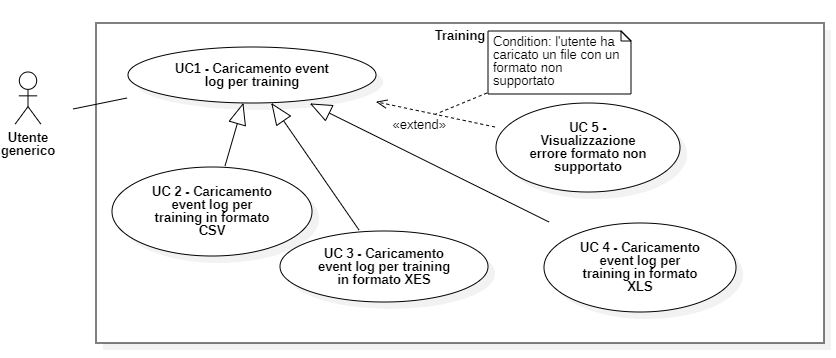
\includegraphics[scale=0.6]{immagini/usecase/cd1.JPG}
    \caption{Casi d'uso relativi al caricamento file di training}
\end{figure}

\subsubsection{UC 1 - Caricamento dell'event log per il training}
\begin{itemize}
	\item \textbf{Attore primario:} Utente generico;
	\item \textbf{Descrizione:} L'utente deve poter caricare l'event log per la fase di training;
	\item \textbf{Scenario principale:} 
		\begin{enumerate}
			\item L'utente seleziona l'event log su cui eseguire il training, in formato CSV (\textbf{UC 2}), XES (\textbf{UC 3}) o XLS (\textbf{UC 4});
			\item L'utente carica l'event log.
		\end{enumerate}
	\item \textbf{Estensioni:} L'utente ha tentato di caricare un event log con formato non supportato e viene mostrato un errore (\textbf{UC 4});
	\item \textbf{Precondizioni:} Non è stato caricato nessun event log su cui effettuare training;
	\item \textbf{Postcondizioni:} L'event log per il training è stato correttamente caricato nel sistema.

\end{itemize}

\subsubsection{UC 2 - Caricamento dell'event log per il training in formato CSV}
\begin{itemize}
	\item \textbf{Attore primario:} Utente generico;
	\item \textbf{Descrizione:} L'utente deve poter caricare l'event log per il training in formato CSV;
	\item \textbf{Scenario principale:} L'utente carica l'event log per il training in formato CSV;
	\item \textbf{Precondizioni:} Non è stato caricato nessun event log su cui effettuare training;
	\item \textbf{Postcondizioni:} L'event log per il training in formato CSV è stato correttamente caricato nel sistema.

\end{itemize}

\subsubsection{UC 3 - Caricamento dell'event log per il training in formato XES}
\begin{itemize}

	\item \textbf{Attore primario:} Utente generico;
	\item \textbf{Descrizione:} L'utente deve poter caricare l'event log per il training in formato XES;
	\item \textbf{Scenario principale:} L'utente carica l'event log per il training in formato XES;
	\item \textbf{Precondizioni:} Non è stato caricato nessun event log su cui effettuare training;
	\item \textbf{Postcondizioni:} L'event log per il training in formato XES è stato correttamente caricato nel sistema.

\end{itemize}



\subsubsection{UC 4 - Caricamento dell'event log per il training in formato XLS}
\begin{itemize}
	\item \textbf{Attore primario:} Utente generico;
	\item \textbf{Descrizione:} L'utente deve poter caricare l'event log per il training in formato XLS;
	\item \textbf{Scenario principale:} L'utente carica l'event log per il training in formato XLS;
	\item \textbf{Precondizioni:} Non è stato caricato nessun event log su cui effettuare training;
	\item \textbf{Postcondizioni:} L'event log per il training in formato XLS è stato correttamente caricato nel sistema.

\end{itemize}



\subsubsection{UC 5 - Visualizzazione errore formato non supportato}
\begin{itemize}
	\item \textbf{Attore primario:} Utente generico;
	\item \textbf{Descrizione:} L'utente deve ricevere un errore in caso venga caricato un event log con formato non supportato
	\item \textbf{Scenario principale:} 
		\begin{enumerate}
			\item L'utente seleziona un event log da caricare con un formato non supportato;
			\item L'utente carica l'event log;
			\item Viene mostrato un messaggio d'errore esplicativo.
		\end{enumerate}
	
	\item \textbf{Precondizioni:} L'utente ha caricato un event log con un formato non supportato;
	\item \textbf{Postcondizioni:} Viene mostrato il messaggio d'errore e l'event log non viene caricato.
\end{itemize}



\begin{figure}[H]
    \centering
    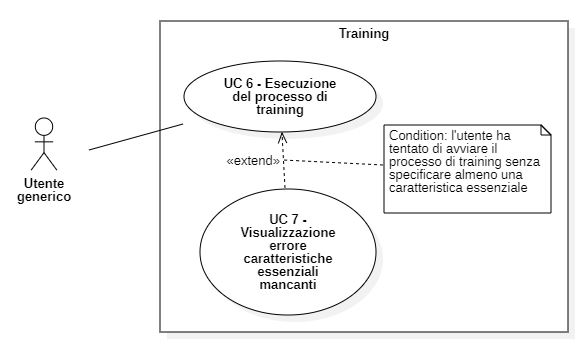
\includegraphics[scale=0.6]{immagini/usecase/cd2.JPG}
    \caption{Casi d'uso relativi al processo di training}
\end{figure}

\subsubsection{UC 6 - Esecuzione del processo di training}
\begin{itemize}
	\item \textbf{Attore primario:} Utente generico;
	\item \textbf{Descrizione:} L'utente deve poter avviare il processo di training;
	\item \textbf{Scenario principale:} 
		\begin{enumerate}
			\item L'utente seleziona le colonne relative alle features dell'event log (\textbf{UC 6.1});
			\item L'utente seleziona il KPI che desidera (\textbf{UC 6.2});		
			\item L'utente seleziona la soglia di frequenza degli outliers che desidera (\textbf{UC 6.3});
			\item L'utente clicca sul pulsante "Start training";
			\item Il processo di training sull'event log caricato e con le caratteristiche selezionate viene avviato:
			\item L'utente visualizza il progresso del processo di training (\textbf{UC 6.4}); 
			\item Al termine del processo l'utente viene notificato;
		\end{enumerate}
	\item \textbf{Estensioni:} Almeno una delle caratteristiche necessarie non è stata specificata e viene mostrato un errore all'utente (\textbf{UC 7});
	\item \textbf{Precondizioni:} L'event log per il training è stato caricato correttamente (\textbf{UC 1});
	\item \textbf{Postcondizioni:} Il processo di training è stato completato con successo. 

\end{itemize}


\begin{figure}[H]
    \centering
    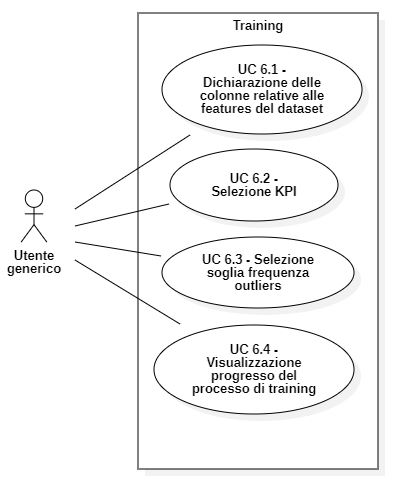
\includegraphics[scale=0.6]{immagini/usecase/cd3.JPG}
    \caption{Casi d'uso relativi al processo di training}
\end{figure}

\subsubsection{UC 6.1 - Dichiarazione delle colonne relative alle features del dataset}
\begin{itemize}
	\item \textbf{Attore primario:} Utente generico;
	\item \textbf{Descrizione:} L'utente deve poter dichiarare quali colonne sono relative a quali features del dataset caricato.
	\item \textbf{Scenario principale:} 
		\begin{enumerate}
			\item L'utente dichiara la colonna relativa alla feature "id" (\textbf{UC 6.1.1});
			\item L'utente dichiara la colonna relativa alla feature "activity" (\textbf{UC 6.1.2});
			\item L'utente dichiara la colonna relativa alla feature "timestamp" (\textbf{UC 6.1.3});
			\item L'utente dichiara la colonna relativa alla feature "resurce" (\textbf{UC 6.1.4}).
		\end{enumerate}
	
	\item \textbf{Precondizioni:} L'event log in formato CSV o XLS è stato caricato correttamente (\textbf{UC 2}, \textbf{UC 4});
	\item \textbf{Postcondizioni:} Il sistema conosce a quale colonna corrisponde ogni feature relative al dataset CSV o XLS caricato.
\end{itemize}

\begin{figure}[H]
    \centering
    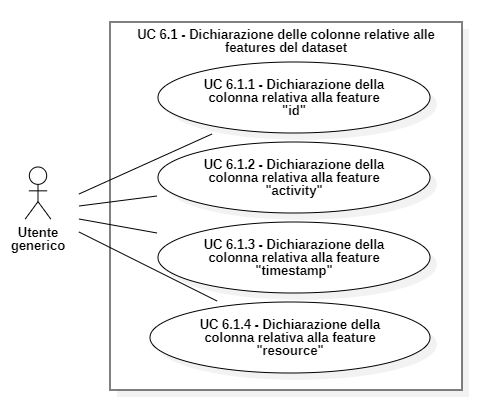
\includegraphics[scale=0.6]{immagini/usecase/cd5.JPG}
    \caption{Casi d'uso relativi alla dichiarazione delle colonne}
\end{figure}

\subsubsection{UC 6.1.1 - Dichiarazione della colonna relativa alla feature "id"}
\begin{itemize}
	\item \textbf{Attore primario:} Utente generico;
	\item \textbf{Descrizione:} L'utente deve poter selezionare la colonna corrispondente alla feature "id".
	\item \textbf{Scenario principale:} 
		\begin{enumerate}
			\item L'utente seleziona il campo relativo alla feature "id";
			\item L'utente dichiara la colonna relativa alla feature "id".
		\end{enumerate}
	\item \textbf{Precondizioni:} L'event log in formato CSV o XLS è stato caricato correttamente (\textbf{UC 2}, \textbf{UC 4});
	\item \textbf{Postcondizioni:} La colonna relativa alla feature "id" è stata dichiarata.
\end{itemize}


\subsubsection{UC 6.1.2 - Dichiarazione della colonna relativa alla feature "activity"}
\begin{itemize}
	\item \textbf{Attore primario:} Utente generico;
	\item \textbf{Descrizione:} L'utente deve poter selezionare la colonna corrispondente alla feature "activity".
	\item \textbf{Scenario principale:} 
		\begin{enumerate}
			\item L'utente seleziona il campo relativo alla feature "activity";
			\item L'utente dichiara la colonna relativa alla feature "activity".
		\end{enumerate}
	\item \textbf{Precondizioni:}  L'event log in formato CSV o XLS è stato caricato correttamente (\textbf{UC 2}, \textbf{UC 4});
	\item \textbf{Postcondizioni:} La colonna relativa alla feature "activity" è stata dichiarata.
\end{itemize}

\subsubsection{UC 6.1.3 - Dichiarazione della colonna relativa alla feature "timestamp"}
\begin{itemize}
	\item \textbf{Attore primario:} Utente generico;
	\item \textbf{Descrizione:} L'utente deve poter selezionare la colonna corrispondente alla feature "timestamp".
	\item \textbf{Scenario principale:} 
		\begin{enumerate}
			\item L'utente seleziona il campo relativo alla feature "timestamp";
			\item L'utente dichiara la colonna relativa alla feature "timestamp".
		\end{enumerate}
	\item \textbf{Precondizioni:}  L'event log in formato CSV o XLS è stato caricato correttamente (\textbf{UC 2}, \textbf{UC 4});
	\item \textbf{Postcondizioni:} La colonna relativa alla feature "timestamp" è stata dichiarata.
\end{itemize}

\subsubsection{UC 6.1.4 - Dichiarazione della colonna relativa alla feature "resource"}
\begin{itemize}
	\item \textbf{Attore primario:} Utente generico;
	\item \textbf{Descrizione:} L'utente deve poter selezionare la colonna corrispondente alla feature "resource".
	\item \textbf{Scenario principale:} 
		\begin{enumerate}
			\item L'utente seleziona il campo relativo alla feature "resource";
			\item L'utente dichiara la colonna relativa alla feature "resource".
		\end{enumerate}
	\item \textbf{Precondizioni:}  L'event log in formato CSV o XLS è stato caricato correttamente (\textbf{UC 2}, \textbf{UC 4});
	\item \textbf{Postcondizioni:} La colonna relativa alla feature "resource" è stata dichiarata.
\end{itemize}


\subsubsection{UC 6.2 - Selezione KPI}
\begin{itemize}
	\item \textbf{Attore primario:} Utente generico;
	\item \textbf{Descrizione:} L'utente deve poter selezionare il KPI che desidera tra quelli disponibili;
	\item \textbf{Scenario principale:} L'utente seleziona il KPI tra:
		\begin{itemize}
			\item "Total time" (\textbf{UC 6.2.1});
			\item "Minimize activity occurence" (\textbf{UC 6.2.2});
			%\item "Maximize activity occurence" (\textbf{UC 5.1.3});
			%\item "Cost" (\textbf{UC 5.3});
		\end{itemize}
	\item \textbf{Precondizioni:} Il file di training è stato caricato correttamente (\textbf{UC 1});
	\item \textbf{Postcondizioni:} Il KPI è stato selezionato.
\end{itemize}

\begin{figure}[H]
    \centering
    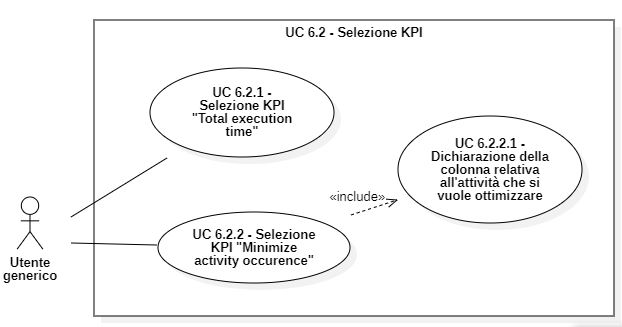
\includegraphics[scale=0.6]{immagini/usecase/cd4.JPG}
    \caption{Casi d'uso relativi alla selezione del KPI}
\end{figure}

\subsubsection{UC 6.2.1 - Selezione KPI "Total time"}
\begin{itemize}
	\item \textbf{Attore primario:} Utente generico;
	\item \textbf{Descrizione:} L'utente deve poter selezionare il KPI "Total time";
	\item \textbf{Scenario principale:} L'utente seleziona il KPI "Total time";
			
	\item \textbf{Precondizioni:} Il file di training è stato caricato correttamente (\textbf{UC 1});
	\item \textbf{Postcondizioni:} Il KPI "Total time" è stato selezionato.
\end{itemize}

%\subsubsection{UC 5.1.2 - Selezione KPI "Maximize activity occurence"}
%\begin{itemize}
%	\item \textbf{Attore primario:} Utente generico;
%	\item \textbf{Descrizione:} L'utente deve poter selezionare il KPI "Maximize activity occurence";
%	\item \textbf{Scenario principale:}
%		\begin{enumerate}
%			\item L'utente seleziona il KPI "Maximize activity occurence";
%			\item L'utente dichiara la colonna relativa all'attività di cui vuole massimizzare le occorrenze (\textbf{UC 5.1.2.1}).
%		\end{enumerate}
%			
%	\item \textbf{Precondizioni:} Il file di training è stato caricato correttamente (\textbf{UC 1});
%	\item \textbf{Postcondizioni:} Il KPI "Maximize activity occurence" è stato selezionato.
%\end{itemize}

\subsubsection{UC 6.2.2 - Selezione KPI "Minimize activity occurence"}
\begin{itemize}
	\item \textbf{Attore primario:} Utente generico;
	\item \textbf{Descrizione:} L'utente deve poter selezionare il KPI "Minimize activity occurence";
	\item \textbf{Scenario principale:}
		\begin{enumerate}
			\item L'utente seleziona il KPI "Minimize activity occurence";
			\item L'utente dichiara la colonna relativa all'attività di cui vuole minimizzare le occorrenze (\textbf{UC 6.2.2.1}).
		\end{enumerate}
			
	\item \textbf{Precondizioni:} Il file di training è stato caricato correttamente (\textbf{UC 1});
	\item \textbf{Postcondizioni:} Il KPI "Minimize activity occurence" è stato selezionato.
\end{itemize}

%\subsubsection{UC 5.3 - Selezione KPI "Cost"}
%\begin{itemize}
%	\item \textbf{Attore primario:} Utente generico;
%	\item \textbf{Descrizione:} L'utente deve poter selezionare il KPI "Cost";
%	\item \textbf{Scenario principale:} L'utente seleziona il KPI "Cost";
%			
%	\item \textbf{Precondizioni:} Il file di training è stato caricato correttamente (\textbf{UC 1});
%	\item \textbf{Postcondizioni:} Il KPI "Cost" è stato selezionato.
%\end{itemize}


\subsubsection{UC 6.2.2.1 - Dichiarazione della colonna relativa all'attività che si vuole ottimizzare}
\begin{itemize}
	\item \textbf{Attore primario:} Utente generico;
	\item \textbf{Descrizione:} L'utente deve poter selezionare la colonna corrispondente all'attività che vuole ottimizzare;
	\item \textbf{Scenario principale:} 
		\begin{enumerate}
			\item L'utente seleziona il campo relativo all'attività che vuole ottimizzare;
			\item L'utente dichiara la colonna relativa all'attività che vuole ottimizzare.
		\end{enumerate}
	\item \textbf{Precondizioni:} 
		\begin{itemize}
			\item Il KPI "Minimize activity occurence" è stato selezionato (\textbf{UC 6.1.3});
			\item La feature "activity" è stata selezionata (\textbf{UC 6.1.2});
		\end{itemize}			
	
	
	\item \textbf{Postcondizioni:} L'attività che si vuole ottimizzare è stata dichiarata.
\end{itemize}


\subsubsection{UC 6.3 - Selezione soglia frequenza outliers}
\begin{itemize}
	\item \textbf{Attore primario:} Utente generico;
	\item \textbf{Descrizione:} L'utente deve avere la possibilità di selezionare la soglia della frequenza degli outliers che desidera;
	\item \textbf{Scenario principale:} L'utente seleziona la soglia che desidera;
	\item \textbf{Estensioni:} Se l'utente non seleziona nessuna soglia viene considerata una soglia di default;
	\item \textbf{Precondizioni:} L'utente ha caricato correttamente il file di training (UC 1);
	\item \textbf{Postcondizioni:} La soglia immessa è stata registrata dal sistema.
\end{itemize}





\subsubsection{UC 6.4 - Visualizzazione progresso del processo di training}
\begin{itemize}
	\item \textbf{Attore primario:} Utente generico;
	\item \textbf{Descrizione:} L'utente deve poter visualizzazione il progresso del processo di training
	\item \textbf{Scenario principale:} L'utente visualizza un indicatore relativo all'attuale progresso del processo di training;
	\item \textbf{Precondizioni:} Il processo di training è stato avviato correttamente (\textbf{UC 6});
	\item \textbf{Postcondizioni:} L'utente è in grado di stimare quanto manca al termine del processo di training.
\end{itemize}


\subsubsection{UC 7 - Visualizzazione errore caratteristiche essenziali mancanti}
\begin{itemize}
	\item \textbf{Attore primario:} Utente generico;
	\item \textbf{Descrizione:} L'utente ha tentanto di avviare il training non avendo inserito una delle caratteristiche essenziali;
	\item \textbf{Scenario principale:}
		\begin{enumerate}
			\item L'utente non ha specificato almeno una tra le seguenti caratteristiche essenziali:
				\begin{itemize}
					\item KPI (\textbf{UC 6.2});
					\item Colonna relativa ad una feature (\textbf{UC 6.1.x});
					\item Attività da ottimizzare (\textbf{UC 6.2.2.1}).
				\end{itemize}
			\item L'utente ha cliccato il pulsante "Start training";
			
		\end{enumerate}
	\item \textbf{Precondizioni:} L'utente ha tentato di avviare il processo di training senza specificare almeno una caratteristica essenziale; 
	\item \textbf{Postcondizioni:} Il processo di training non viene avviato e all'utente viene visualizzato un errore esplicativo.
\end{itemize}


\subsubsection{UC 8 - Download del process model generato dal processo di training}
\begin{itemize}
	\item \textbf{Attore primario:} Utente generico;
	\item \textbf{Descrizione:} L'utente deve poter fare il download dei file del process model generato del processo di training;
	\item \textbf{Scenario principale:}
		\begin{enumerate}
			\item L'utente clicca il pulsante "Download training files";
			\item I file che compongono il process model vengono scaricati.
		\end{enumerate}
	\item \textbf{Precondizioni:} L'utente ha terminato con successo il processo di training (\textbf{UC 6}); 
	\item \textbf{Postcondizioni:} L'utente ha scaricato i file del process model.
\end{itemize}



%% -------------------------
%% ---- RUNNING PHASE ------
%% -------------------------

\begin{figure}[H]
    \centering
    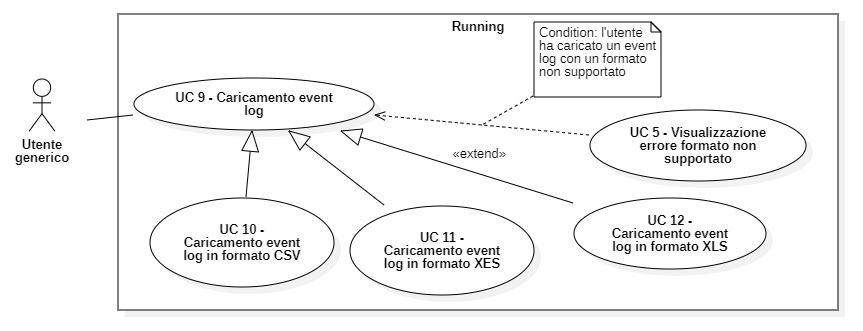
\includegraphics[scale=0.6]{immagini/usecase/cd6.JPG}
    \caption{Casi d'uso relativi al caricamento del file di log}
\end{figure}


\subsubsection{UC 9 - Caricamento dell'event log per il calcolo delle raccomandazioni}
\begin{itemize}
	\item \textbf{Attore primario:} Utente generico;
	\item \textbf{Descrizione:} L'utente deve poter caricare l'event log per il calcolo delle raccomandazioni;
	\item \textbf{Scenario principale:} 
		\begin{enumerate}
			\item L'utente seleziona l'event log per il calcolo delle raccomandazioni in formato CSV (\textbf{UC 10}), XES (\textbf{UC 11}) o XLS (\textbf{UC 12});
			\item L'utente carica l'event log selezionato.
		\end{enumerate}
	\item \textbf{Estensioni:} L'utente ha tentato di caricare un event log con formato non supportato e viene mostrato un errore (\textbf{UC 5});
		
	\item \textbf{Precondizioni:} La fase di training è stata completata (\textbf{UC 6}) oppure l'utente ha caricato un modello già allenato (\textbf{UC 19});
	\item \textbf{Postcondizioni:} L'event log per la running phase è stato correttamente caricato nel sistema.
\end{itemize}

\subsubsection{UC 10 - Caricamento dell'event log per il calcolo delle raccomandazioni in formato CSV}
\begin{itemize}
	\item \textbf{Attore primario:} Utente generico;
	\item \textbf{Descrizione:} L'utente deve poter caricare l'event log per il calcolo delle raccomandazioni in formato CSV;
	\item \textbf{Scenario principale:} L'utente carica l'event log per il calcolo delle raccomandazioni in formato CSV;
	\item \textbf{Precondizioni:} Non è stato caricato nessun event log per il calcolo delle raccomandazioni;
	\item \textbf{Postcondizioni:} L'event log per il calcolo delle raccomandazioni in formato XES è stato correttamente caricato nel sistema.
\end{itemize}

\subsubsection{UC 11 - Caricamento dell'event log per il calcolo delle raccomandazioni in formato XES}
\begin{itemize}
	\item \textbf{Attore primario:} Utente generico;
	\item \textbf{Descrizione:} L'utente deve poter caricare l'event log per il calcolo delle raccomandazioni in formato XES;
	\item \textbf{Scenario principale:} L'utente carica l'event log per il calcolo delle raccomandazioni in formato XES;
	\item \textbf{Precondizioni:} Non è stato caricato nessun event log per il calcolo delle raccomandazioni;
	\item \textbf{Postcondizioni:} L'event log per il calcolo delle raccomandazioni in formato XES è stato correttamente caricato nel sistema.
\end{itemize}

\subsubsection{UC 12 - Caricamento dell'event log per il calcolo delle raccomandazioni in formato XLS}
\begin{itemize}
	\item \textbf{Attore primario:} Utente generico;
	\item \textbf{Descrizione:} L'utente deve poter caricare l'event log per il calcolo delle raccomandazioni in formato XLS;
	\item \textbf{Scenario principale:} L'utente carica l'event log per il calcolo delle raccomandazioni in formato XLS;
	\item \textbf{Precondizioni:} Non è stato caricato nessun event log per il calcolo delle raccomandazioni;
	\item \textbf{Postcondizioni:} L'event log per il calcolo delle raccomandazioni in formato XLS è stato correttamente caricato nel sistema.
\end{itemize}

\begin{figure}[H]
    \centering
    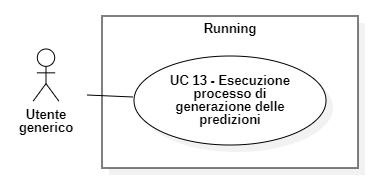
\includegraphics[scale=0.6]{immagini/usecase/cd7.JPG}
    \caption{Caso d'uso relativo al processo di generazione delle raccomandazioni}
\end{figure}

\subsubsection{UC 13 - Esecuzione processo di generazione delle raccomandazioni}
\begin{itemize}
	\item \textbf{Attore primario:} Utente generico;
	\item \textbf{Descrizione:} L'utente deve poter avviare il processo di generazione delle raccomandazioni;
	\item \textbf{Scenario principale:} 
		\begin{enumerate}
			\item L'utente clicca sul pulsante "Generate recommendations";
			\item Il processo di generazione delle predizioni sull'event log caricato si avvia;
			\item L'utente visualizza il progresso del processo di generazione delle raccomandazioni (\textbf{UC 13.1});
			\item Al termine del processo l'utente viene notificato.
		\end{enumerate}
	\item \textbf{Precondizioni:} L'event log per il calcolo delle raccomandazioni è stato caricato correttamente (\textbf{UC 9});
	\item \textbf{Postcondizioni:} Il processo di generazione delle raccomandazioni è stato completato con successo. 
\end{itemize}

\begin{figure}[H]
    \centering
    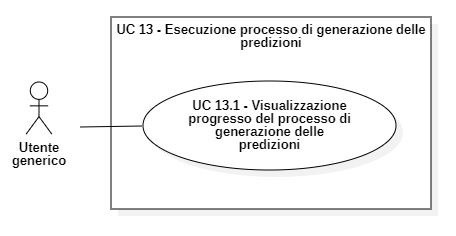
\includegraphics[scale=0.6]{immagini/usecase/cd8.JPG}
    \caption{Caso d'uso relativo alla visualizzazione del progresso relativo al processo di generazione delle raccomandazioni}
\end{figure}

\subsubsection{UC 13.1 - Visualizzazione progresso del processo di generazione delle raccomandazioni}
\begin{itemize}
	\item \textbf{Attore primario:} Utente generico;
	\item \textbf{Descrizione:} L'utente deve poter visualizzazione il progresso del processo di generazione delle raccomandazioni
	\item \textbf{Scenario principale:} L'utente visualizza un indicatore relativo all'attuale progresso del processo di generazione delle raccomandazioni;
	\item \textbf{Precondizioni:} Il processo di generazione delle raccomandazioni è stato avviato correttamente (\textbf{UC 13});
	\item \textbf{Postcondizioni:} L'utente è in grado di stimare quanto manca al termine del processo di generazione delle raccomandazioni.
\end{itemize}

\begin{figure}[H]
    \centering
    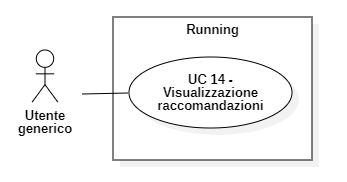
\includegraphics[scale=0.6]{immagini/usecase/cd9.JPG}
    \caption{Caso d'uso relativo alla visualizzazione delle raccomandazioni}
\end{figure}

\subsubsection{UC 14 - Visualizzazione raccomandazioni}
\begin{itemize}
	\item \textbf{Attore primario:} Utente generico;
	\item \textbf{Descrizione:} L'utente deve essere in grado di visualizzare le raccomandazioni generate;
	\item \textbf{Scenario principale:} L'utente visualizza l'insieme delle raccomandazioni generate.

	\item \textbf{Sottocasi:}
		\begin{itemize}
			\item L'utente visualizza la raccomandazione relativa alla singola traccia (\textbf{UC 14.1});
		\end{itemize}
		
	\item \textbf{Estensioni:} L'utente può riordinare le raccomandazioni secondo alcuni ordinamenti predefiniti (\textbf{UC 14.2})
	\item \textbf{Precondizioni:} Il processo di generazione delle predizioni è completato (\textbf{UC 13});
	\item \textbf{Postcondizioni:} L'utente ha visualizzato le predizioni.
\end{itemize}

\begin{figure}[H]
    \centering
    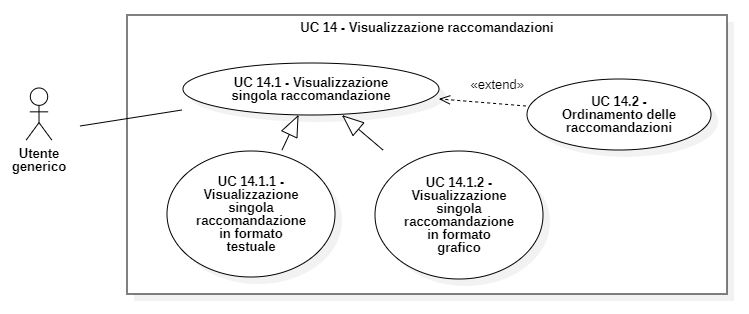
\includegraphics[scale=0.6]{immagini/usecase/cd10.JPG}
    \caption{Casi d'uso relativi alla visualizzazione della singola raccomandazione}
\end{figure}

\subsubsection{UC 14.1 - Visualizzazione raccomandazioni per una singola traccia}
\begin{itemize}
	\item \textbf{Attore primario:} Utente generico;
	\item \textbf{Descrizione:} L'utente deve poter visualizzare le raccomandazioni per una singola traccia;
	\item \textbf{Scenario principale:}
		\begin{enumerate}
			\item L'utente seleziona la traccia a cui è interessato;
			\item L'utente visualizza le raccomandazioni (per la singola traccia) in formato testuale (\textbf{UC 14.1.1}) e grafico (\textbf{UC 14.1.2}).
		\end{enumerate}
	\item \textbf{Precondizioni:} L'utente sta svolgendo l'attività di visualizzazione;
	\item \textbf{Postcondizioni:} L'utente ha visualizzato le raccomandazioni di suo interesse.
\end{itemize}

\subsubsection{UC 14.1.1 - Visualizzazione singola raccomandazione in formato testuale}
\begin{itemize}
	\item \textbf{Attore primario:} Utente generico;
	\item \textbf{Descrizione:} L'utente deve poter visualizzare le migliori raccomandazioni (fino ad un massimo di 3) e la predizione dell'attività in corso, con i corrispettivi KPI espressi in maniera testuale;
	\item \textbf{Scenario principale:}
		\begin{enumerate}
			\item L'utente visualizza le 3 migliori raccomandazioni e la predizione dell'attività in corso; 
			\item L'utente visualizza i KPI predetti delle attività raccomandate e visualizza il KPI della predizione sulla base dell'attività in corso.
		\end{enumerate}
	\item \textbf{Precondizioni:} L'utente sta svolgendo l'attività di visualizzazione;
	\item \textbf{Postcondizioni:} L'utente ha visualizzato la singola raccomandazione di suo interesse.
\end{itemize}

\subsubsection{UC 14.1.2 - Visualizzazione singola raccomandazione in formato grafico}
\begin{itemize}
	\item \textbf{Attore primario:} Utente generico;
	\item \textbf{Descrizione:} L'utente deve poter visualizzare i KPI della migliore raccomandazione in forma grafica;
	\item \textbf{Scenario principale:} L'utente visualizza un grafico che rappresenta i KPI della migliore attività raccomandata;
	\item \textbf{Precondizioni:} L'utente sta svolgendo l'attività di visualizzazione;
	\item \textbf{Postcondizioni:} L'utente ha visualizzato la singola predizione di suo interesse tramite un grafico.
\end{itemize}


\subsubsection{UC 14.2 - Ordinamento delle raccomandazioni}
\begin{itemize}
	\item \textbf{Attore primario:} Utente generico;
	\item \textbf{Descrizione:} L'utente può riordinare l'insieme di tutte le raccomandazioni secondo alcuni ordinamenti predefiniti;
	\item \textbf{Scenario principale:} 
	\begin{itemize}
		\item L'utente sceglie in tipo di ordinamento tra:
			\begin{itemize}
				\item "Delta from maximum": Le raccomandazioni sono riordinate in ordine decrescente di variazione;
				\item "Delta from minimum": Le raccomandazioni sono riordinate in ordine crescente di variazione;
				\item "Maximize": Le raccomandazioni sono riordinate in ordine decrescente; 
				\item "Minimize": Le raccomandazioni sono riordinate in ordine crescente;
			\end{itemize}
		\item L'utente visualizza le raccomandazioni con il nuovo ordinamento;
	\end{itemize}
	\item \textbf{Precondizioni:} L'utente sta visualizzando tutte le raccomandazioni generate;
	\item \textbf{Postcondizioni:} L'utente visualizza le raccomandazioni riordinate secondo l'ordinamento scelto;
\end{itemize}

\subsubsection{UC 15 - Ricerca traccia per id}
\begin{itemize}
	\item \textbf{Attore primario:} Utente generico;
	\item \textbf{Descrizione:} L'utente deve poter ricercare le tracce per id
	\item \textbf{Scenario principale:} 
		\begin{enumerate}
			\item L'utente seleziona il campo di ricerca;
			\item L'utente digita l'id della traccia a cui è interessato;
			\item L'utente può selezionare la traccia ricercata;
		\end{enumerate}
	\item \textbf{Precondizioni:} L'utente sta svolgendo l'attività di ricerca;
	\item \textbf{Postcondizioni:} L'utente ha trovato la traccia corrispondente all'id a cui era interessato.
\end{itemize}

\subsubsection{UC 16 - Ricerca traccia tramite grafico}
\begin{itemize}
	\item \textbf{Attore primario:} Utente generico;
	\item \textbf{Descrizione:} L'utente deve poter ricercare le tracce selezionandole in un grafico che le rappresenta; 
	\item \textbf{Scenario principale:} 
		\begin{enumerate}
			\item L'utente visualizza un grafico che mostra tutte le tracce;
			\item L'utente clicca sulla traccia a cui è interessato;
			\item La traccia viene selezionata;
		\end{enumerate}
	\item \textbf{Precondizioni:} L'utente sta svolgendo l'attività di ricerca;
	\item \textbf{Postcondizioni:} L'utente ha selezionato una traccia a cui è interessato.
\end{itemize}

\begin{figure}[H]
    \centering
    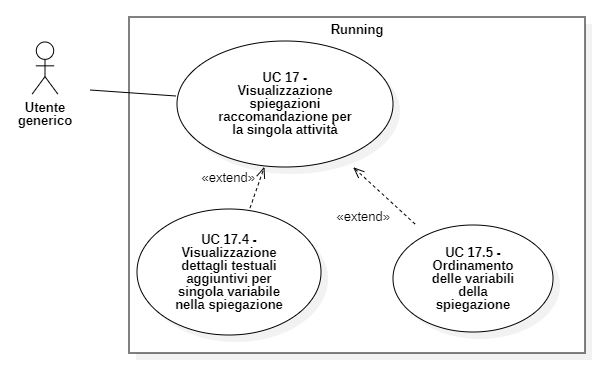
\includegraphics[scale=0.6]{immagini/usecase/cd11.JPG}
    \caption{Caso d'uso relativo alla visualizzazione delle spiegazioni}
\end{figure}

\subsubsection{UC 17 - Visualizzazione spiegazioni singola raccomandazione}
\begin{itemize}
	\item \textbf{Attore primario:} Utente generico;
	\item \textbf{Descrizione:} L'utente deve poter visualizzare le spiegazioni per ogni raccomandazione di una singola traccia
	\item \textbf{Scenario principale:} 
		\begin{enumerate}
			\item L'utente seleziona la traccia a cui è interessato (\textbf{UC 15}, \textbf{UC 16});
			\item L'utente seleziona la raccomandazione di cui vuole visualizzare la spiegazione (\textbf{UC 17.1});
			\item L'utente seleziona la quantità di variabili che vuole visualizzare nella spiegazione(\textbf{UC 17.2});
			\item L'utente visualizza la spiegazione in formato grafico (\textbf{UC 17.3}); 
		\end{enumerate}
	\item \textbf{Estensioni}: 
	\begin{itemize}
		\item Una volta visualizzate le spiegazioni l'utente può selezionare una singola variabile spiegata per poter ottenere dettagli testuali aggiuntivi (\textbf{UC 17.4});
		\item L'utente può riordinare le variabili delle spiegazioni secondo ordinamenti predefiniti (\textbf{17.5});
	\end{itemize}

	\item \textbf{Precondizioni:} L'utente sta svolgendo l'attività di visualizzazione e il processo di generazione delle raccomandazioni è completato (\textbf{UC 13});
	\item \textbf{Postcondizioni:} L'utente ha visualizzato le spiegazioni relative ad una attività tra quelle raccomandate per una traccia di suo interesse.
\end{itemize}

\begin{figure}[H]
    \centering
    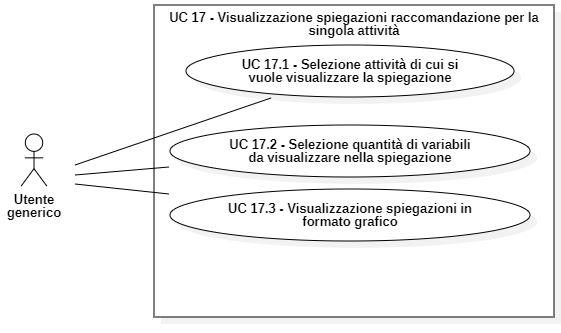
\includegraphics[scale=0.6]{immagini/usecase/cd12.JPG}
    \caption{Casi d'uso relativi alla visualizzazione di una singola raccomandazione}
\end{figure}

\subsubsection{UC 17.1 - Selezione attività di cui si vuole visualizzare la spiegazione}
\begin{itemize}
	\item \textbf{Attore primario:} Utente generico;
	\item \textbf{Descrizione:} L'utente deve poter selezionare l'attività raccomandata di cui vuole visualizzare la spiegazione;
	\item \textbf{Scenario principale:} L'utente seleziona l'attività raccomandata che desidera;

	\item \textbf{Precondizioni:} L'utente sta svolgendo l'attività di visualizzazione delle raccomandazioni;
	\item \textbf{Postcondizioni:} Il sistema ha registrato l'attività a cui l'utente è interessato di vedere le spiegazioni.
\end{itemize}

\subsubsection{UC 17.2 - Selezione quantità di variabili da visualizzare nella spiegazione}
\begin{itemize}
	\item \textbf{Attore primario:} Utente generico;
	\item \textbf{Descrizione:} L'utente deve poter visualizzare quante variabili visualizzare per la spiegazione;
	\item \textbf{Scenario principale:}
	\begin{enumerate}
			\item L'utente seleziona il campo di selezione quantità;
			\item L'utente sceglie la quantità desiderata.
		\end{enumerate}
	
	\item \textbf{Precondizioni:} L'utente sta svolgendo l'attività di visualizzazione delle raccomandazioni;
	\item \textbf{Postcondizioni:} Il sistema ha registrato la quantità di spiegazione che l'utente è interessato a visualizzare
\end{itemize}

\subsubsection{UC 17.3 - Visualizzazione spiegazione in formato grafico}
\begin{itemize}
	\item \textbf{Attore primario:} Utente generico;
	\item \textbf{Descrizione:} L'utente deve poter visualizzare un grafico che rappresenta le singole variazioni relative alle variabili da spiegare;
	\item \textbf{Scenario principale:} L'utente visualizza un grafico in cui sono rappresentati le singole variazioni alle variabili prese in considerazione;
	
	\item \textbf{Precondizioni:}
	\begin{itemize}
			\item l'utente ha selezionato l'attività di cui vuole visualizzare la spiegazione (\textbf{UC 17.1}) 
	 		\item l'utente ha selezionato la quantità di variabili che desidera visualizzare nella spiegazione 	(\textbf{UC 17.2})
	 	\end{itemize}
	\item \textbf{Postcondizioni:} L'utente ha visualizzato le spiegazione in formato grafico;
\end{itemize}


\subsubsection{UC 17.4 - Visualizzazione dettagli testuali aggiuntivi per singola variabile nella spiegazione}
\begin{itemize}
	\item \textbf{Attore primario:} Utente generico;
	\item \textbf{Descrizione:} L'utente può selezionare una singola variabile per ottenere una spiegazione testuale più dettagliata;
	\item \textbf{Scenario principale:} 
		\begin{itemize}
			\item L'utente seleziona la variabile della spiegazione sui cui vuole avere dei dettagli aggiuntivi;
			\item L'utente visualizza i dettagli aggiuntivi relativi alla variabile selezionata in forma testuale;
		\end{itemize}
	
	\item \textbf{Precondizioni:} L'utente sta visualizzando la spiegazione di una raccomandazione;
	\item \textbf{Postcondizioni:} L'utente ha ottenuto dettaglia aggiuntivi su una singola variabile della spiegazione;
\end{itemize}

\subsubsection{UC 17.5 - Ordinamento delle variabili della spiegazione}
\begin{itemize}
	\item \textbf{Attore primario:} Utente generico;
	\item \textbf{Descrizione:} L'utente può riordinare le variabili della spiegazione secondo alcuni ordinamenti predefiniti;
	\item \textbf{Scenario principale:} 
	\begin{itemize}
		\item L'utente sceglie in tipo di ordinamento tra:
			\begin{itemize}
				\item "Delta from maximum": Le variabili della spiegazione sono riordinate in ordine decrescente di variazione;
				\item "Delta from minimum": Le variabili della spiegazione sono riordinate in ordine crescente di variazione;
			\end{itemize}
		\item L'utente visualizza le spiegazioni con il nuovo ordinamento;
	\end{itemize}
	\item \textbf{Precondizioni:} L'utente sta visualizzando la spiegazione di una raccomandazione;
	\item \textbf{Postcondizioni:} L'utente visualizza le variabili della spiegazione riordinate secondo l'ordinamento scelto;
\end{itemize}


\subsubsection{UC 18 - Inserimento nome esperimento}
\begin{itemize}
	\item \textbf{Attore primario:} Utente generico;
	\item \textbf{Descrizione:} L'utente deve poter nominare l'esperimento effettuato;
	\item \textbf{Scenario principale:} L'utente inserisce il nome che preferisce per l'esperimento;
	\item \textbf{Estensioni:} Se l'utente non inserisce nessun nome viene inserito un nome di default; 
	\item \textbf{Precondizioni:} L'utente non ha ancora iniziato il processo di training (\textbf{UC 6})
	\item \textbf{Postcondizioni:} Il sistema ha registrato la preferenza dell'utente.
\end{itemize}

\subsubsection{UC 19 - Caricamento modello già precedentemente allenato}
\begin{itemize}
	\item \textbf{Attore primario:} Utente generico;
	\item \textbf{Descrizione:} L'utente deve poter caricare un modello già allenato (permettendo di saltare la fase di training)
	\item \textbf{Scenario principale:}
		\begin{enumerate}
			\item L'utente seleziona il campo relativo al caricamento di modelli già allenati;
			\item L'utente seleziona un modello da caricare;
			\item L'utente clicca su "Load model".
		\end{enumerate}
	\item \textbf{Precondizioni:} L'utente deve aver a disposizione dei modelli già allenati; 
	\item \textbf{Postcondizioni:} L'utente può procedere all'inserimento dell'event log per la generazione delle raccomandazioni con il modello caricato.
\end{itemize}

\clearpage
\section{Tracciamento dei requisiti}
Da un'attenta analisi dei requisiti e degli use case effettuata sul progetto è stata stilata la tabella che traccia i requisiti in rapporto agli use case. 
\\
Sono stati individuati diversi tipi di requisiti e si è quindi fatto utilizzo di un codice identificativo per distinguerli.
\\
Il codice dei requisiti è così strutturato: 
\\
\centerline{\textbf{R[Tipologia][Classificazione]-[Identificativo]}}

\begin{itemize}
	\item \textbf{Tipologia}:
	\begin{itemize}
		\item \textbf{F}: Funzionale;
		\item \textbf{NF}; Non funzionale;
	\end{itemize}
	\item \textbf{Classificazione}:
	\begin{itemize}
		\item \textbf{O}: Obbligatorio;
		\item \textbf{F}: Facoltativo;
	\end{itemize}
	\item \textbf{Identificativo}: codice univoco incrementale per ogni requisito con valore iniziale pari ad 1.
\end{itemize}


%\begin{enumerate}
%	\item[R =] requisito
%    \item[F =] funzionale
%    \item[Q =] qualitativo
%    \item[V =] di vincolo
%    \item[N =] obbligatorio (necessario)
%    \item[D =] desiderabile
%    \item[Z =] opzionale
%\end{enumerate}
%Nelle tabelle \ref{tab:requisiti-funzionali}, \ref{tab:requisiti-qualitativi} e \ref{tab:requisiti-vincolo} sono riassunti i requisiti e il loro tracciamento con gli use case delineati in fase di analisi.

%\newpage

%\begin{table}
%\caption{Tabella del tracciamento dei requisti funzionali}
%\label{tab:requisiti-funzionali}
\begin{longtable}{cp{8cm}ll}
\hline
\hline
\textbf{Requisito} & \textbf{Descrizione} &  \textbf{Rilevanza} & \textbf{Fonte}\\
\hline
RF1 & L'interfaccia permette all'utente di caricare un event log per il processo di training & Obbligatorio & UC1 \\
\hline
RF2 & L'interfaccia permette all'utente di caricare un event log per il processo di training in formato CSV & Obbligatorio & UC2 \\
\hline
RF3 & L'interfaccia permette all'utente di caricare un event log per il processo di training in formato XES & Obbligatorio & UC3 \\
\hline
RF4 & L'interfaccia permette all'utente di caricare un event log per il processo di training in formato XLS & Obbligatorio & UC4 \\
\hline
RF5 & L'interfaccia visualizza un'errore se l'utente carica un event log con formato sono supportato & Obbligatorio & UC5 \\
\hline
RF6 & L'interfaccia permette all'utente di avviare il processo di training & Obbligatorio & UC6 \\
\hline
RF6.1 & Se il formato dell'event log per il training caricato è CSV o XLS, L'interfaccia permette all'utente di dichiarare le colonne relative alle features necessarie & Obbligatorio & UC6.1 \\
\hline 
RF6.1.1 & L'interfaccia permette all'utente di dichiarare la colonna relativa alla feature "ID" & Obbligatorio & UC6.1.1 \\
\hline
RF6.1.2 & L'interfaccia permette all'utente di dichiarare la colonna relativa alla feature "Activity" & Obbligatorio & UC6.1.2 \\
\hline
RF6.1.3 & L'interfaccia permette all'utente di dichiarare la colonna relativa alla feature "Timestamp" & Obbligatorio & UC6.1.3 \\
\hline
RF6.1.4 & L'interfaccia permette all'utente di dichiarare la colonna relativa alla feature "Resource" & Obbligatorio & UC6.1.4 \\
\hline
RF6.2 & L'interfaccia permette all'utente di selezionare il KPI a cui è interessato & Obbligatorio & UC6.2 \\
\hline
RF6.2.1 & L'interfaccia permette all'utente di selezionare il KPI "Total time" & Obbligatorio & UC6.2.1 \\
\hline
RF6.2.2 & L'interfaccia permette all'utente di selezionare il KPI "Minimize activity occurrence" & Obbligatorio & UC6.2.2 \\
\hline
RF6.2.2.1 & Se il KPI "Minimize activity occurrence" è stato selezionato, l'interfaccia permette all'utente di dichiarare l'attività che vuole ottimizzare & Obbligatorio & UC6.2.2.1 \\
\hline
RF6.3 & L'interfaccia permette all'utente di selezionare la soglia di frequenza degli outliers & Obbligatorio & UC6.3 \\
\hline
RF6.4 & L'interfaccia permette all'utente di visualizzare il progresso del processo di training & Obbligatorio & UC6.4 \\
\hline
RF7 & L'interfaccia visualizza un errore se l'utente non inserisce almeno una delle caratteristiche essenziali per il processo di training & Obbligatorio & UC7 \\
\hline
RF8 & L'interfaccia permette all'utente di effettuare il download dei file del process model generato dal processo di training & Obbligatorio & UC8 \\
\hline
RF9 & L'interfaccia permette all'utente di caricare l'event log per il processo di generazione delle raccomandazioni & Obbligatorio & UC9 \\
\hline
RF10 & L'interfaccia permette all'utente di caricare l'event log per il processo di generazione delle raccomandazioni in formato CSV & Obbligatorio & UC10 \\
\hline
RF11 & L'interfaccia permette all'utente di caricare l'event log per il processo di generazione delle raccomandazioni in formato XES & Obbligatorio & UC11 \\
\hline
RF12 & L'interfaccia permette all'utente di caricare l'event log per il processo di generazione delle raccomandazioni in formato XLS & Obbligatorio & UC12 \\
\hline
RF13 & L'interfaccia permette all'utente di avviare il processo di generazione delle raccomandazioni & Obbligatorio & UC13 \\
\hline
RF13 & L'interfaccia permette all'utente di avviare il processo di generazione delle raccomandazioni & Obbligatorio & UC13 \\
\hline
RF13.1 & L'interfaccia permette all'utente di visualizzare il progresso del processo di generazione delle raccomandazioni & Obbligatorio & UC13.1 \\
\hline
RF14 & L'interfaccia permette all'utente di visualizzare le raccomandazioni generate & Obbligatorio & UC14 \\
\hline
RF14.1 & L'interfaccia permette all'utente di visualizzare le raccomandazioni relative ad una singola traccia & Obbligatorio & UC14.1 \\
\hline
RF14.1.1 & L'interfaccia permette all'utente di visualizzare le raccomandazioni relative ad una singola traccia in formato testuale & Obbligatorio & UC14.1.1 \\
\hline
RF14.1.2 & L'interfaccia permette all'utente di visualizzare le raccomandazioni relative ad una singola traccia in formato grafico & Obbligatorio & UC14.1.2 \\
\hline
RF14.2 & L'interfaccia permette all'utente di riordinare l'insieme delle raccomandazioni generate & Obbligatorio & UC14.2 \\
\hline
RF15 & L'interfaccia permette all'utente di ricercare una traccia tramite id & Obbligatorio & UC15 \\
\hline
RF16 & L'interfaccia permette all'utente di ricercare una traccia tramite grafico & Obbligatorio & UC16 \\
\hline
RF17 & L'interfaccia permette all'utente di visualizzare le spiegazioni di una singola raccomandazione & Obbligatorio & UC17 \\
\hline
RF17.1 & L'interfaccia permette all'utente di selezionare l'attività raccomandata di cui vuole visualizzare la spiegazione & Obbligatorio & UC17.1 \\
\hline
RF17.2 & L'interfaccia permette all'utente di selezionare la qualtità di variabili che vuole visualizzare nella spiegazione & Obbligatorio & UC17.2 \\
\hline
RF17.3 & L'interfaccia permette all'utente di visualizzare la spiegazione in formato grafico & Obbligatorio & UC17.3 \\
\hline
RF17.4 & L'interfaccia permette all'utente di visualizzare dettagli testuali aggiuntivi per ogni singola variabile della spiegazione & Obbligatorio & UC17.4 \\
\hline
RF17.5 & L'interfaccia permette all'utente di riordinare le variabili della spiegazione  & Obbligatorio & UC17.5 \\
\hline
RF18 & L'interfaccia permette all'utente di definire il nome da dare all'esperimento effettuato  & Obbligatorio & UC18 \\
\hline
RF19 & L'interfaccia permette all'utente caricare nel sistema un modello già allenato in precedenza  & Obbligatorio & UC19 \\
\hline
\hline
\caption{Tabella del tracciamento dei requisti funzionali}
\end{longtable}
%\end{table}



\begin{longtable}{cp{8cm}ll}
\hline
\hline
\textbf{Requisito} & \textbf{Descrizione} &  \textbf{Rilevanza} & \textbf{Fonte}\\
\hline
RNF1 & L'interfaccia deve funzionare correttamente nelle ultime attuali versioni dei sistemi operativi Windows, MacOS e Ubuntu & Obbligatorio & Committente \\
\hline
RNF2 & L'interfaccia deve essere sviluppata usando il framework Dash & Obbligatorio & Scelta interna \\
\hline
RNF3 & L'interfaccia deve essere sviluppata in modalità wizard (cioè una procedura step by step) & Obbligatorio & Committente \\
\hline
RNF4 & L'interfaccia deve poter essere utilizzata da più utenti indipendenti contemporaneamente & Desiderabile & D01 \\
\hline
RNF5 & Devono essere presenti test di unità per l'interfaccia grafica & Obbligatorio & O06 \\

\hline
\hline
\caption{Tabella del tracciamento dei requisti non funzionali}
\end{longtable}